\chapter{Medotologia e Resultados}\label{cap:CnptDsng}
\section{Desenvolvimento do código Arduino RTU}
O programa realiza a conversão de valores decimais em binários, lê o status de um botão e o valor de um potenciômetro somado com um setpoint. 

Para aplicação do modo de transmissão MODBUS RTU no Arduíno, foi utilizada a biblioteca \verb|“SimpleModbusSlave.h”|, onde o arduino foi configurado como escravo, sendo assim, o computador o mestre.

A função \verb|modbus_configure| é responsável pela configuração dos parâmetros da comunicação, foram escolhidos os valores de baud-rate sendo iguais a 9600, o formato de dados como \verb|SERIAL_N2|, que equivale ao tamanho da palavra de dados, e o endereço do arduino como sendo 1.

O Arduíno se comunica com o usuário por meio da interface gráfica, dessa forma as variáveis de entrada do programa são o valor para ser convertido em binário, um \textit{setpoint} para ser adicionado ao valor do potenciômetro lido e o sinal de botão pressionado, proveniente de um botão físico. 

O programa possui 3 saídas: o valor do número decimal convertido para binário e mostrado num sistema físico de 3 leds; o mesmo valor já convertido para binário mostrado também na interface gráfica e o valor lido pelo potenciômetro mais o \textit{setpoint} informado.O programa está mostrado à seguir:


\begin{lstlisting}[language=Arduino]
#include <SimpleModbusSlave.h>

int LED1 = 8; //Definicao das portas dos LEDs
int LED2 = 6;
int LED3 = 4;
int botao = 2;



enum //Enumera as variaveis  que serao utilizadas para comunicacao com o Elipse E3
{
BINARIO, // recebe o valor em decimal para ser convertido em binario
LED_1, 
LED_2, 
LED_3,
POTENCIOMETRO, //Recebe o valor do sensor LDR; primeiro componente que o E3 ira \"reconhecer\"(N4 = 01)
SETPOINT, //Recebe o valor decimal; (N4 = 02)
SETPOT,
BOTAO,  
HOLDING_REGS_SIZE //Identifica a quantidade de holdingRegs que estao sendo utilizados no programa.
};

unsigned int holdingRegs[HOLDING_REGS_SIZE]; //Variavel criada para manipulacao dos registradores que foram criados. 

int num = 0;
int setpoint;

void setup() {

modbus_configure(&Serial, 9600, SERIAL_8N2, 1, 2, HOLDING_REGS_SIZE, holdingRegs); //Determina os parametros necessarios para estabelecer a conexao via comunicacao serial utilizando MODBUS.
//9600 = velocidade da transmissao dos dados; SERIAL_8N2 = formato do pacote utilizado no MODBUS; 1 = identificacao do escravo.

modbus_update_comms(9600, SERIAL_8N2, 1); //Funcao tambem responsavel pela comunicacao via MODBUS; 

pinMode (LED1, OUTPUT); //Modos de operacao dos LEDs (saida)
pinMode (LED2, OUTPUT);
pinMode (LED3, OUTPUT);
pinMode (botao, INPUT);
}


void loop() {

modbus_update(); // Funcao utilizada para a atulizacao dos valores dos registradores declarados (V_LDR, V_LED...)

holdingRegs[POTENCIOMETRO] = analogRead(A0); //Le-se a informacao presente na porta analogica A0 (Sensor LDR)
setpoint = holdingRegs[SETPOINT];
holdingRegs[SETPOT] = setpoint + analogRead(A0);
holdingRegs[BOTAO] = digitalRead(botao);

switch(holdingRegs[BINARIO]) {
case 0:
digitalWrite(LED1, LOW);
digitalWrite(LED2, LOW);
digitalWrite(LED3, LOW);
holdingRegs[LED_1] = 0;
holdingRegs[LED_2] = 0;
holdingRegs[LED_3] = 0;
break;
case 1:
digitalWrite(LED1, HIGH);
digitalWrite(LED2, LOW);
digitalWrite(LED3, LOW);
holdingRegs[LED_1] = 1;
holdingRegs[LED_2] = 0;
holdingRegs[LED_3] = 0;
break;
case 2:
digitalWrite(LED1, LOW);
digitalWrite(LED2, HIGH);
digitalWrite(LED3, LOW);
holdingRegs[LED_1] = 0;
holdingRegs[LED_2] = 1;
holdingRegs[LED_3] = 0;
break;
case 3:
digitalWrite(LED1, HIGH);
digitalWrite(LED2, HIGH);
digitalWrite(LED3, LOW);
holdingRegs[LED_1] = 1;
holdingRegs[LED_2] = 1;
holdingRegs[LED_3] = 0;
break;
case 4:
digitalWrite(LED1, LOW);
digitalWrite(LED2, LOW);
digitalWrite(LED3, HIGH);
holdingRegs[LED_1] = 0;
holdingRegs[LED_2] = 0;
holdingRegs[LED_3] = 1;
break;
case 5:
digitalWrite(LED1, HIGH);
digitalWrite(LED2, LOW);
digitalWrite(LED3, HIGH);
holdingRegs[LED_1] = 1;
holdingRegs[LED_2] = 0;
holdingRegs[LED_3] = 1;
break;
case 6:
digitalWrite(LED1, LOW);
digitalWrite(LED2, HIGH);
digitalWrite(LED3, HIGH);
holdingRegs[LED_1] = 0;
holdingRegs[LED_2] = 1;
holdingRegs[LED_3] = 1;
break; 
case 7:
digitalWrite(LED1, HIGH);
digitalWrite(LED2, HIGH);
digitalWrite(LED3, HIGH);
holdingRegs[LED_1] = 1;
holdingRegs[LED_2] = 1;
holdingRegs[LED_3] = 1;
break;
}
}
\end{lstlisting}

\section{Desenvolvimento do código Arduino TCP}
Assim como o código anterior,este programa realiza a conversão de valores decimais em binários, lê o status de um botão e o valor de um potenciômetro somado com um \textit{setpoint}, a comunicação entre o Arduíno e Elipse é feita por meio do protocolo TCP.
Para aplicação do modo de transmissão MODBUS TCP no arduino, foram utilizada as bibliotecas \verb|“SPI.h “|, \verb|“Ethernet.h”| e \verb|"Mudbus.h"|.

A biblioteca \verb|“SPI.h”| é responsável pela comunicação serial entre o \textit{shield} Ethernet e Arduíno, a biblioteca \verb|“Ethernet.h”| realiza a configuração dos parâmetros de ethernet e pela conectividade a rede e a biblioteca \verb|“Mudbus.h”| configura protocolo modbus da comunicação. Para a comunicação o arduino foi configurado como servidor, recebendo as requisições do computador, que funciona como cliente.

A função \verb|Ethernet.begin| é responsável pela configuração dos parâmetros a comunicação, foram escolhidos os valores de IP sendo igual $192.168.1.1$, o gateway igual a $192.168.1.1$ e endereço de subrede de $255.255.255.0$.

O programa está ilustrado a seguir, apresentando as mesmas entradas e saídas do anterior.
\begin{lstlisting}[language=Arduino]
#include <SPI.h> 
#include <Ethernet.h>
#include \"Mudbus.h\"

Mudbus Mb;
//Function codes 1(read coils), 3(read registers), 5(write coil), 6(write register)
//signed int Mb.R[0 to 125] and bool Mb.C[0 to 128] MB_N_R MB_N_C
//Port 502 (defined in Mudbus.h) MB_PORT

int botao = 8;
int LED1 = 7; //Definicao das portas dos LEDs
int LED2 = 6;
int LED3 = 5;
int setpoint;


void setup(){
uint8_t mac[]     = { 0x90, 0xA2, 0xDA, 0x00, 0x51, 0x06 };
uint8_t ip[]      = { 192, 168, 1, 10 };
uint8_t gateway[] = { 192, 168, 1, 1 };
uint8_t subnet[]  = { 255, 255, 255, 0 };
Ethernet.begin(mac, ip,gateway, subnet);
//With the last update of Industrial Shields boards it\'s not necessary to use function pinMode() 


pinMode (LED1, OUTPUT); //Modos de operacao dos LEDs (saida)
pinMode (LED2, OUTPUT);
pinMode (LED3, OUTPUT);
pinMode (botao, INPUT);
}

void loop(){
Mb.Run(); //Update the values of Mb.R and Mb.C every loop cycle

switch(Mb.R[0]) {
case 0:
digitalWrite(LED1, LOW);
digitalWrite(LED2, LOW);
digitalWrite(LED3, LOW);
Mb.R[1] = 0;
Mb.R[2] = 0;
Mb.R[3] = 0;
break;
case 1:
digitalWrite(LED1, HIGH);
digitalWrite(LED2, LOW);
digitalWrite(LED3, LOW);
Mb.R[1] = 1;
Mb.R[2] = 0;
Mb.R[3] = 0;
break;
case 2:
digitalWrite(LED1, LOW);
digitalWrite(LED2, HIGH);
digitalWrite(LED3, LOW);
Mb.R[1] = 0;
Mb.R[2] = 1;
Mb.R[3] = 0;
break;
case 3:
digitalWrite(LED1, HIGH);
digitalWrite(LED2, HIGH);
digitalWrite(LED3, LOW);
Mb.R[1] = 1;
Mb.R[2] = 1;
Mb.R[3] = 0;
break;
case 4:
digitalWrite(LED1, LOW);
digitalWrite(LED2, LOW);
digitalWrite(LED3, HIGH);
Mb.R[1] = 0;
Mb.R[2] = 0;
Mb.R[3] = 1;
break;
case 5:
digitalWrite(LED1, HIGH);
digitalWrite(LED2, LOW);
digitalWrite(LED3, HIGH);
Mb.R[1] = 1;
Mb.R[2] = 0;
Mb.R[3] = 1;
break;
case 6:
digitalWrite(LED1, LOW);
digitalWrite(LED2, HIGH);
digitalWrite(LED3, HIGH);
Mb.R[1] = 0;
Mb.R[2] = 1;
Mb.R[3] = 1;
break; 
case 7:
digitalWrite(LED1, HIGH);
digitalWrite(LED2, HIGH);
digitalWrite(LED3, HIGH);
Mb.R[1] = 1;
Mb.R[2] = 1;
Mb.R[3] = 1;
break;
}


Mb.R[4] = analogRead(A0);
setpoint = Mb.R[5];

Mb.R[6] = Mb.R[4] + setpoint;

//  if( digitalRead(botao)){
//
//    Mb.R[7] = 1;
//  }
//  else{
//    Mb.R[7] = 0;
//  }
Mb.R[7] = digitalRead(botao);
}
\end{lstlisting}
\section{Configuração do computador}
Para comunicar o computador e o Arduíno via Ethernet é preciso criar uma rede local entre eles, como mostrado anteriormente, o Arduíno foi configurado para um IP de $192.168.1.10$ e sub-máscara de 255.255.255.00, o rede do computador foi configurado com o IP $192.168.1.23$ com máscara $255.255.255$.0 o mesmo estara na mesma rede com o Arduíno e assim podendo trocar informações.
\begin{figure}[H]
	\centering
	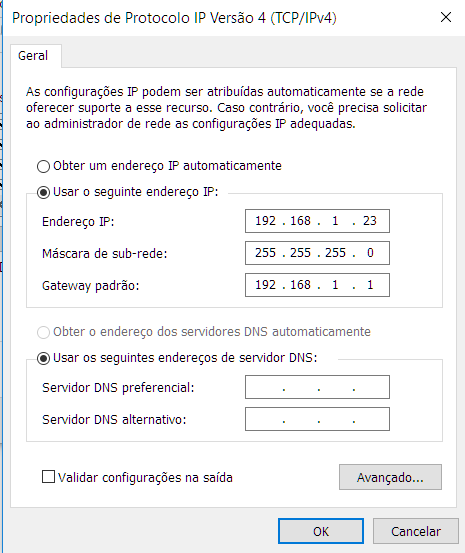
\includegraphics[width=.6\textwidth]{configTCP-PC.PNG}
	\caption{Configuração do computador para comunicação TCP}
	\label{fig:tcp_config1}
	%\source{Fornecido junto com os pontos}
\end{figure}
\section{Comunicação Elipse/Arduino utilizando o modo RTU}
Para realizar a comunicação entre o elipse e o arduino foi necessário o uso de um \textit{Driver} para as duas aplicações,no modo RTU e TCP. Ao abrir a janela de configuração do Driver RTU, foram adicionados duas funções contendo como mostra na figura \ref{fig:rtu_config1}, foi selecionado tambem que o Modbus mode seria RTU. 
Na aba \textit{setup}, ilustrado na figura \ref{fig:rtu_config2}, foi selecionado a camada física “Serial” e o restante Default. As etapa da configuração estão mostradas a seguir: 

\begin{figure}[H]
	\centering
	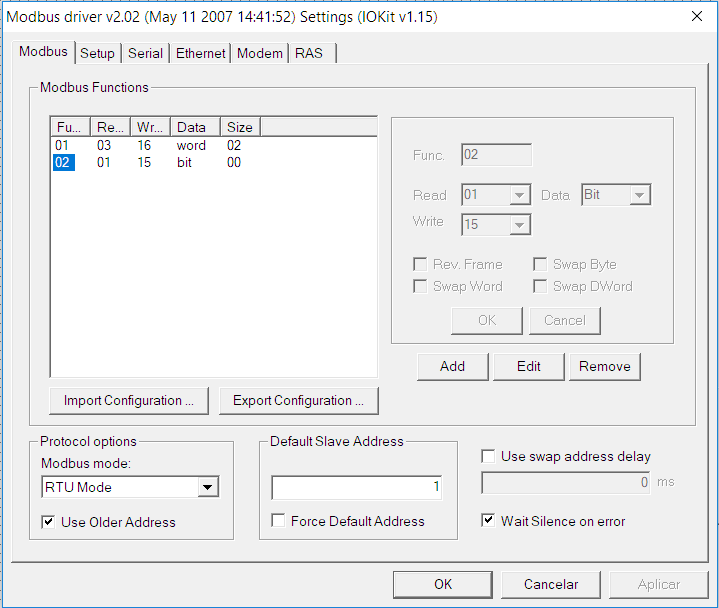
\includegraphics[width=.6\textwidth]{configRTU.PNG}
	\caption{Etapa 1 da configuração RTU}
	\label{fig:rtu_config1}
	%\source{Fornecido junto com os pontos}
\end{figure}

\begin{figure}[H]
	\centering
	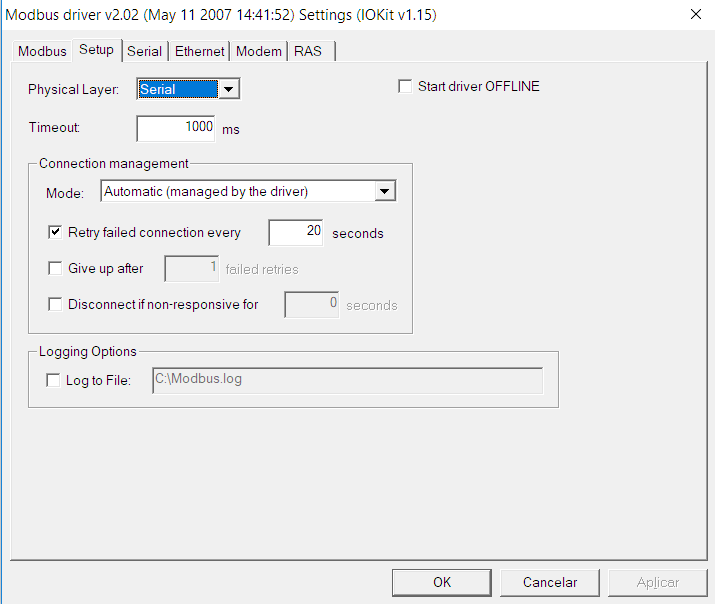
\includegraphics[width=.6\textwidth]{configRTU2.PNG}
	\caption{Etapa 2 da configuração RTU}
	\label{fig:rtu_config2}
	%\source{Fornecido junto com os pontos}
\end{figure}

Após selecionar a camada física Serial, a aba serial pode ser configurada. Nela é configurado a \textit{com port} referente a com na qual o Arduíno esta conectado, juntamente com a configuração de \textit{baud-rate} para 9600, data bits para 8, bit paridade “nenhum e o \textit{stop} bits para 1, como foi configurado no código Arduíno.

\begin{figure}[H]
	\centering
	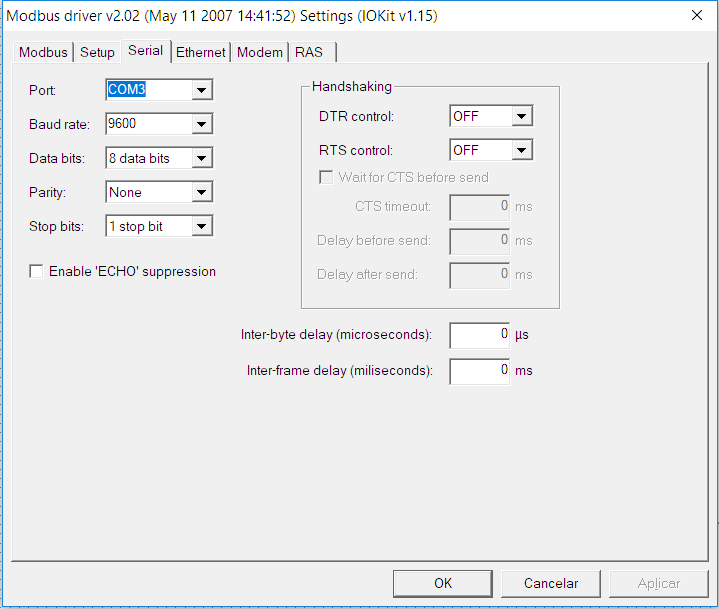
\includegraphics[width=.6\textwidth]{configRTU3.PNG}
	\caption{Etapa 3 da configuração RTU}
	\label{fig:rtu_config3}
	%\source{Fornecido junto com os pontos}
\end{figure}

\section{Comunicação Elipse/Arduino utilizando o modo TCP}
O driver TCP foi configurado de forma parecida ao modo RTU, na aba Modbus única diferença é o modo modbus para \verb|“modubus TCP”|, como mostra a figura \ref{fig:tcp_config1}:
\begin{figure}[H]
	\centering
	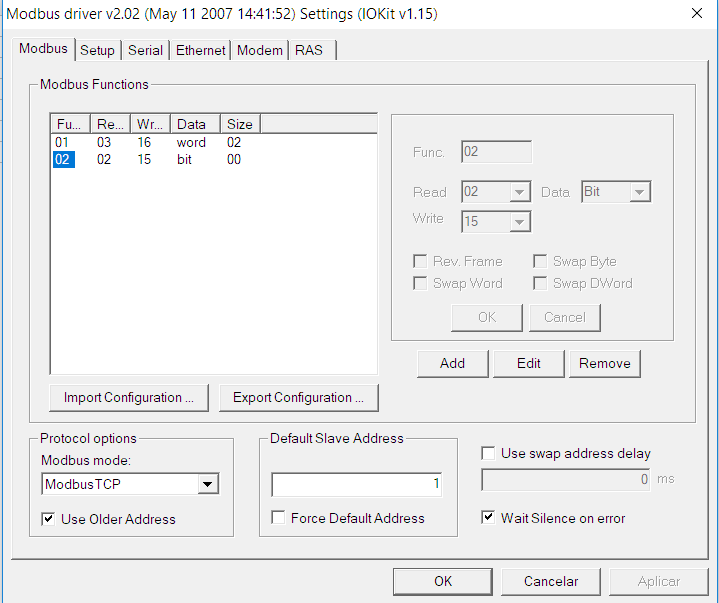
\includegraphics[width=.6\textwidth]{configTCP1.PNG}
	\caption{Etapa 1 da configuração TCP}
	\label{fig:tcp_config1}
	%\source{Fornecido junto com os pontos}
\end{figure}
Na aba “setup”, a camada fisica foi selecionada “ethernet”,como mostra a figura \ref{fig:tcp_config2}:
\begin{figure}[H]
	\centering
	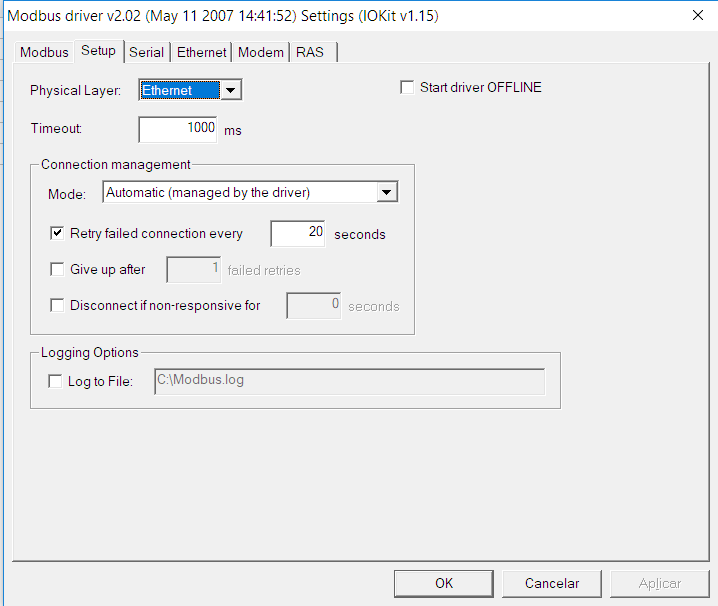
\includegraphics[width=.6\textwidth]{configTCP2.PNG}
	\caption{Etapa 2 da configuração TCP}
	\label{fig:tcp_config2}
	%\source{Fornecido junto com os pontos}
\end{figure}
Na aba \verb|“ethernet”|, no campo \verb|“transport”| foi escolhdio TCP/IP, nos campo IP e \textit{port} foram colocados os mesmos valores configurados no arduino.

\begin{figure}[H]
	\centering
	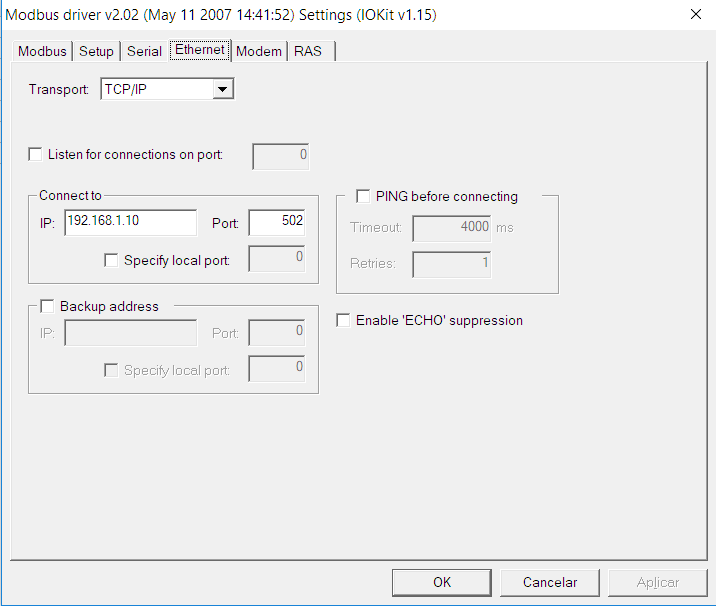
\includegraphics[width=.6\textwidth]{configTCP3.PNG}
	\caption{Etapa 3 da configuração TCP}
	\label{fig:tcp_config3}
	%\source{Fornecido junto com os pontos}
\end{figure}
\section{Configuração das \textit{tags} no Elipse}
Para cada driver, a configuração das tags de comunicação se diferenciou pelo os IDs de cada variável que é representado nas figuras à seguir como a coluna $P4$. A coluna $P1$ representa a configuração do escravo que participará da comunicação,onde na comunicação com o arduino, se adotou o valor de $P1= 1$. $P2$ mostra a função utilizada na configuração do driver, $P3$ indica a utilização de memória estendida. Foi utilizada a função 1 de HoldingRegs, assim $P2= 1$ e não se utilizará a memória extendida, assim $P3 =0$.
\begin{figure}[H]
	\centering
	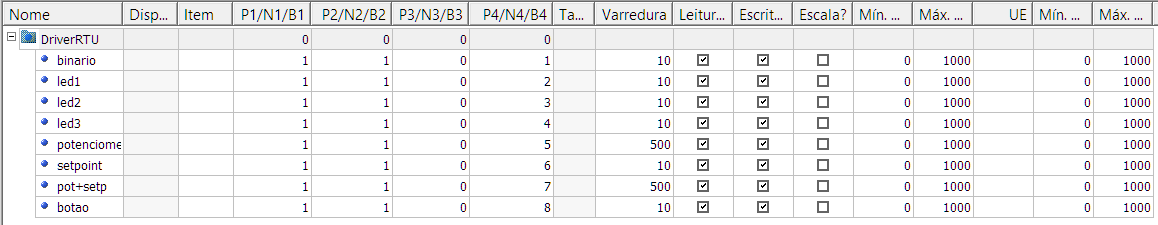
\includegraphics[width=1\textwidth]{configRTU0.PNG}
	\caption{Driver RTU}
	\label{fig:driver_rtu}
	%\source{Fornecido junto com os pontos}
\end{figure}

\begin{figure}[H]
	\centering
	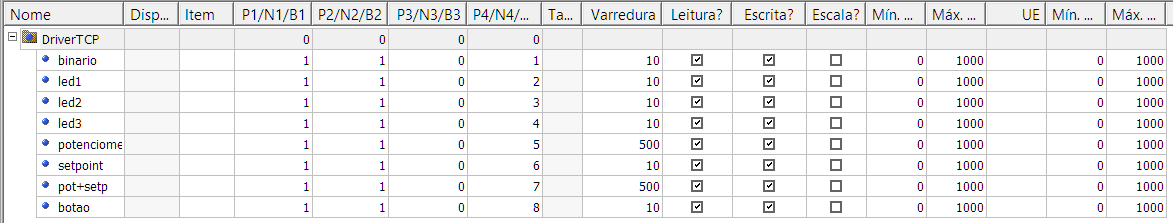
\includegraphics[width=1\textwidth]{configTCP0.PNG}
	\caption{Driver TCP}
	\label{fig:driver_tcp}
	%\source{Fornecido junto com os pontos}
\end{figure}
\section{Interface Gráfica}
A interface gráfica recebe o número para ser convertido em binário e o \textit{offset}
 que será adicionado ao valor do potenciômetro. Cada campo foi relacionado com as \textit{tags} de comunicação do driver mostradas anteriormente, buscou-se desenvolver uma interface simples, os \textit{screenshots} estão mostrados à seguir:

\begin{figure}[H]
	\centering
	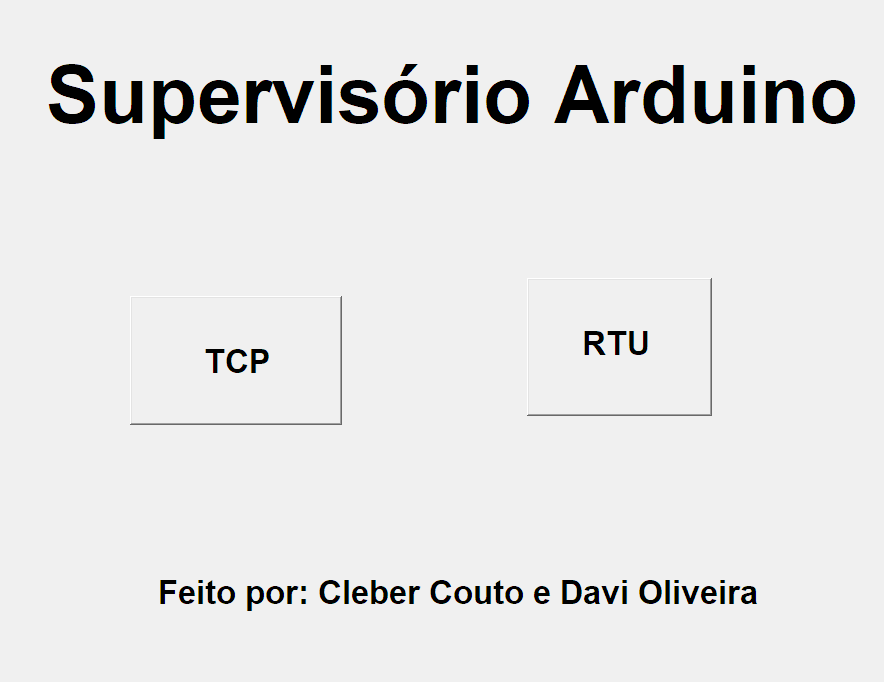
\includegraphics[width=.6\textwidth]{telainterface1.PNG}
	\caption{Tela de seleção do modo de comunicação}
	\label{fig:tela1}
	%\source{Fornecido junto com os pontos}
\end{figure}
\begin{figure}[H]
	\centering
	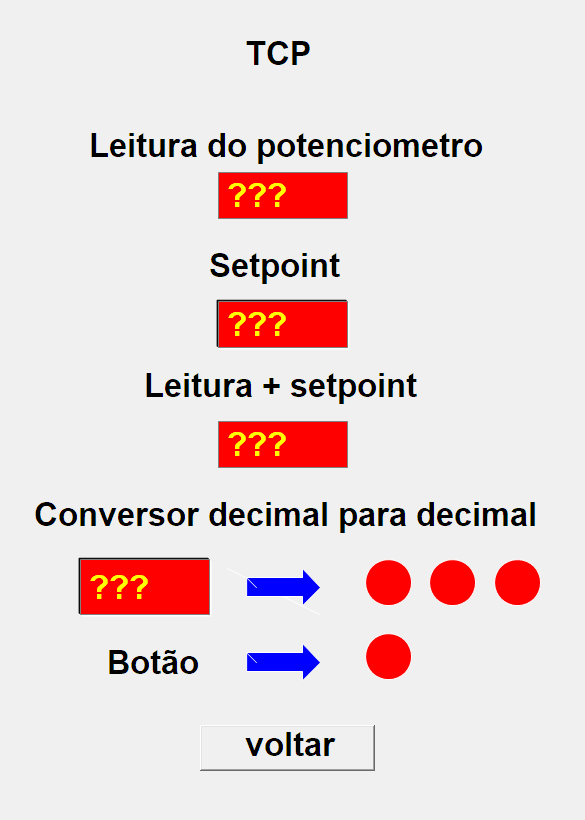
\includegraphics[width=.5\textwidth]{telainterface2.PNG}
	\caption{Tela comunicação TCP}
	\label{fig:tela_tcp}
	%\source{Fornecido junto com os pontos}
\end{figure}
\begin{figure}[H]
	\centering
	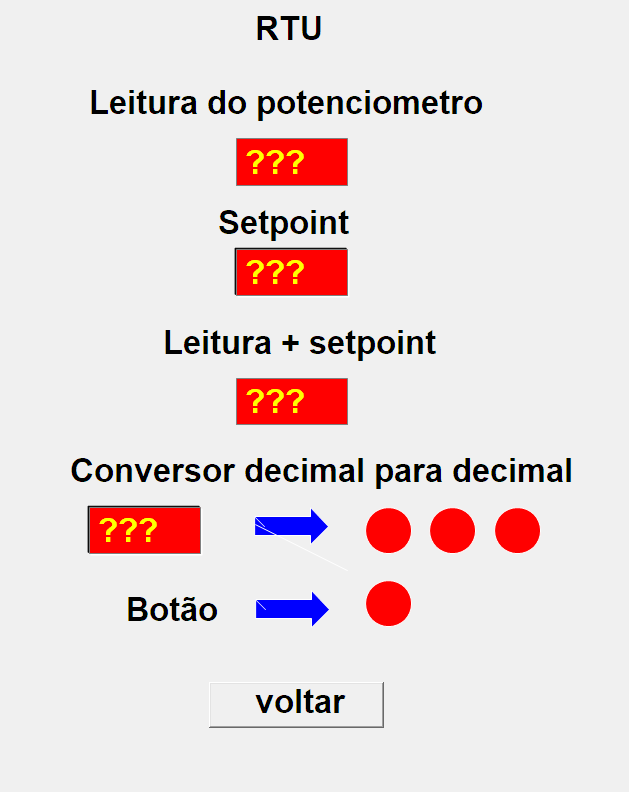
\includegraphics[width=.5\textwidth]{telainterface3.PNG}
	\caption{Tela comunicação RTU}
	\label{fig:tela_rtu}
	%\source{Fornecido junto com os pontos}
\end{figure}
 

